%----------------------------------------------------------------------------
\section[Terv]{Alkalmazás terve}
%----------------------------------------------------------------------------

\subsection[A fő komponens]{Fő komponens: optikai folyam}
%----------------------------------------------------------------------------

\begin{frame}{Optikai folyam}

\begin{itemize}
\item vektormező: a \textbf{képpontok elmozdulása} egyik képről a másikra
\item Gunnar Farnebäck algoritmusa
\item $\rightarrow$ \textbf{párosítás}
\end{itemize}

\centering
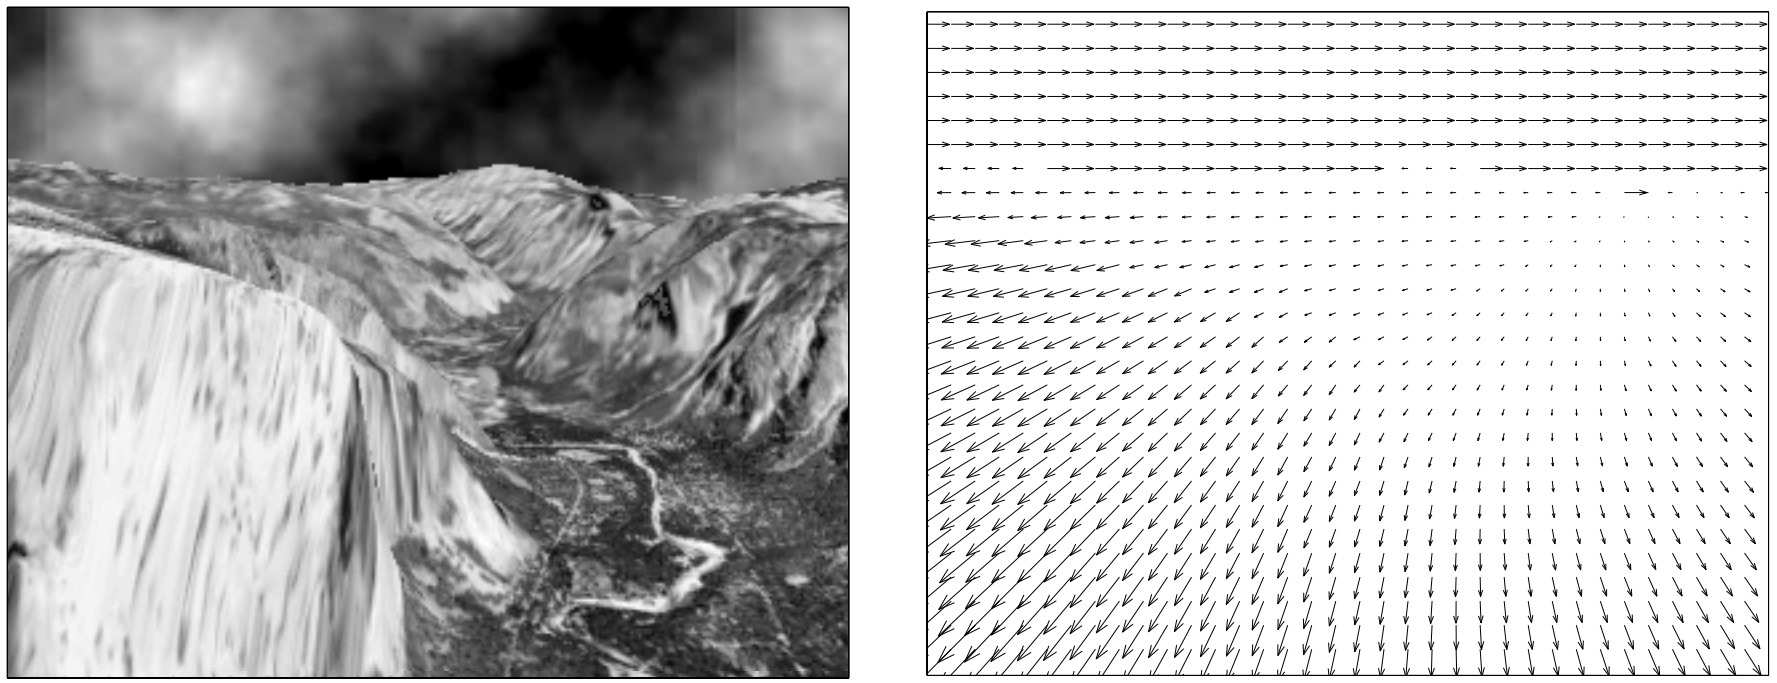
\includegraphics[width=300pt]{figures/farneback.png}

\end{frame}

\subsection[Megvalósított logika]{Megvalósított logika folyamábrája}
%----------------------------------------------------------------------------

\begin{frame}{Folyamatábra}

\pgfdeclarelayer{background}
\pgfdeclarelayer{foreground}
\pgfsetlayers{background,main,foreground}

\centering

\resizebox{0.65\textwidth}{!}{%
\begin{tikzpicture}[->,>=stealth',shorten >=1pt,auto]
\tikzset{
box/.style={draw, rectangle, text width=12em, minimum height=2.5em, text centered},
plain/.style={text width=12em, text centered},
line/.style = {-,shorten >=0pt},
graybox/.style = {box, gray}
}

\node[plain] (Cam1) {1. kamera};

\node[graybox] (Calib1) [below of=Cam1] {Kalibrálás};

\node[box] (GetFrames1) [below of=Calib1,yshift=-1.5em] {Aktuális képkocka lekérése};

\node[box] (FgMask1) [below of=GetFrames1,yshift=-1.5em] {Előtér maszkok meghatározása};

\draw (Calib1) -- (GetFrames1);
\draw (GetFrames1) -- (FgMask1);



\node[plain] (Cam2) [right of=Cam1,xshift=14em] {2. kamera};

\node[graybox] (Calib2) [below of=Cam2] {Kalibrálás};

\node[box] (GetFrames2) [below of=Calib2,yshift=-1.5em] {Aktuális képkocka lekérése};

\node[box] (FgMask2) [below of=GetFrames2,yshift=-1.5em] {Előtér maszkok meghatározása};

\draw (Calib2) -- (GetFrames2);
\draw (GetFrames2) -- (FgMask2);


\node[box] (Obj12) [below of=FgMask1,xshift=8.25em,yshift=-2.5em] {Objektumok detektálása a képpárokon};
 
\draw (FgMask1) |- (Obj12);
\draw (FgMask2) |- (Obj12);


\node[box] (OF12) [below of=Obj12,yshift=-1.5em] {Optikai folyam meghatározása};
 
\draw (Obj12) -- (OF12);


\node[box] (Triangle12) [below of=OF12,yshift=-1.5em] {Háromszögelés};

\draw (OF12) -- (Triangle12);

\node[box] (Contour) [below of=Triangle12,yshift=-1.5em] {Nézőpontból\\ projekció + kontúr};

\draw (Triangle12) -- (Contour);


\begin{pgfonlayer}{background}
    \path (Cam1.north west)+(-0.5,0.5) node (a) {};
    \path (FgMask1.south east)+(+0.5,-0.5) node (b) {};
    \path[rounded corners, draw=black!50, dashed] (a) rectangle (b);
\end{pgfonlayer}

\begin{pgfonlayer}{background}
    \path (Cam2.north west)+(-0.5,0.5) node (a) {};
    \path (FgMask2.south east)+(+0.5,-0.5) node (b) {};
    \path[rounded corners, draw=black!50, dashed] (a) rectangle (b);
\end{pgfonlayer}

\end{tikzpicture}
}

\end{frame}


%----------------------------------------------------------------------------
\section[Lépések]{A főbb lépések}
%----------------------------------------------------------------------------

\subsection*{}
%----------------------------------------------------------------------------

\begin{frame}{Kamerák kalibrálása}

\begin{itemize}
\item Torzítás kiküszöbölése
\item Pozíciójuk meghatározása a világ-koordinátarendszerben
\end{itemize}

\begin{figure}[tbh]
\centering
\begin{subfigure}[b]{.49\linewidth}
	\centering
	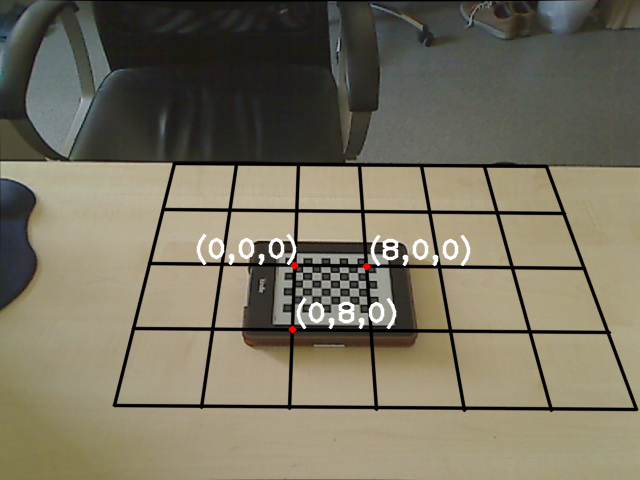
\includegraphics[width=140pt]{figures/pose0_180.png}
	\caption{Bal oldali kamera képe}
  \end{subfigure}
\begin{subfigure}[b]{.49\linewidth}
	\centering
	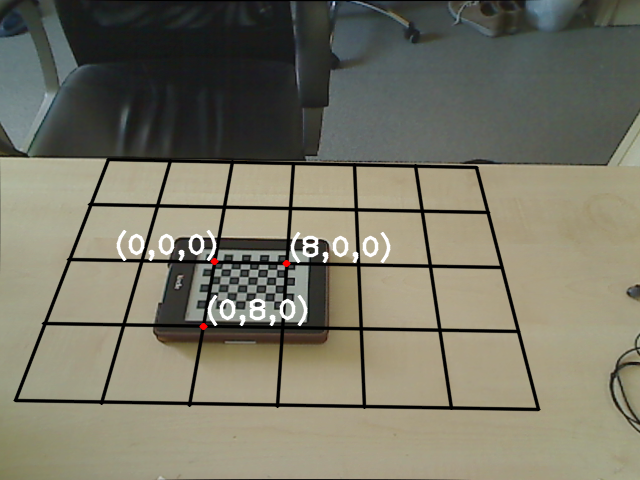
\includegraphics[width=140pt]{figures/pose1_180.png}
	\caption{Jobb oldali kamera képe}
  \end{subfigure}
%\caption{Világ-koordinátarendszer jelölése a képeken \label{fig:pose}}
\end{figure}

\end{frame}


\begin{frame}{Mozgó objektumok meghatározása -- előtér maszkok}

\begin{itemize}
\item {\color{gray} Háttér-modell építés}
\item Optikai folyam
\end{itemize}

\begin{figure}[tbh]
\centering
\begin{subfigure}[b]{.49\linewidth}
	\centering
	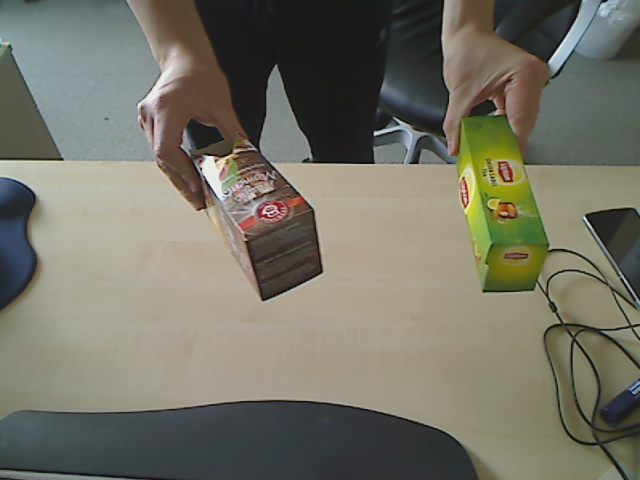
\includegraphics[width=140pt]{figures/frame_ofmask_107.png}
	\caption{Aktuális képkocka}
  \end{subfigure}
\begin{subfigure}[b]{.49\linewidth}
	\centering
	
\includegraphics[width=140pt]{figures/mask_ofmask_107.png}
	\caption{Számított maszk}
  \end{subfigure}
%\caption{Előző és az aktuális képkockából számított előtér maszk}
\end{figure}

\end{frame}


\begin{frame}{Objektumok azonosítása a képpárokon}
\begin{enumerate}
    \item jellegzetes pontok kijelölése (ORB)
    \item ezek párosítása (brute-force)
    \item blobok összerendelése (többségi döntés)
\end{enumerate}

\vspace{10pt}
\centering
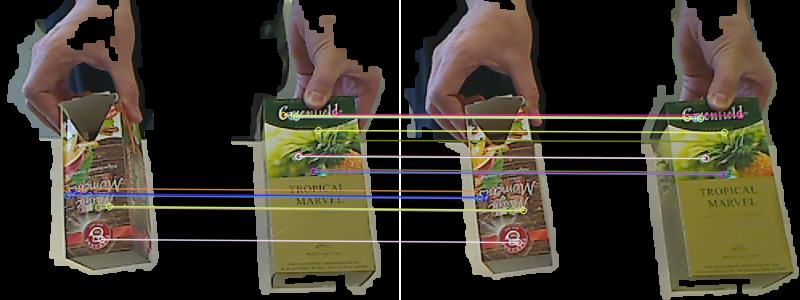
\includegraphics[width=300pt]{figures/multi_obj_matches.png}

\end{frame}


\begin{frame}{Optikai folyam segítségével sűrű pontpárosítás}
\begin{itemize}
\item eltolás minimalizálása a két kép között
\item textúrázatlanság és kitakarás kezelése
\end{itemize}

\begin{figure}[tbh]
\centering
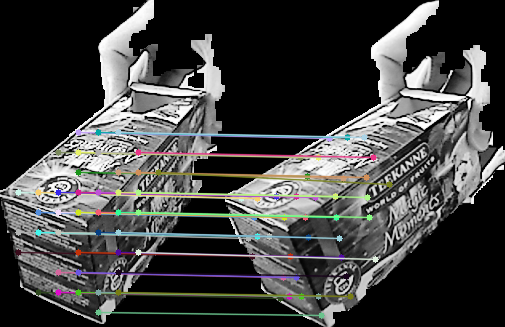
\includegraphics[width=200pt]{figures/vis_full.png}
%\caption{Néhány párosítás kiemelve (kb. 16 800 vektor)}
\end{figure}


\end{frame}


\begin{frame}{Objektumok pontjainak meghatározása a térben}

\begin{itemize}
\item kamerák helyzete ismert
\item pontpárosítások alapján $\rightarrow$ pontonként \textbf{háromszögelés}
\end{itemize}

\vspace{10pt}
\centering
\tdplotsetmaincoords{60}{130}
\resizebox{0.8\textwidth}{!}{%
\begin{tikzpicture}[line join = round, line cap = round, >=triangle 45, tdplot_main_coords]
  
  \coordinate (O) at (0, 0, 0);
  
  % kocka
  
  \coordinate (C1) at (-4.5, -2, 1);
  \coordinate (C2) at (-4.5, -1, 1);
  \coordinate (C3) at (-4.5, -1, 2);
  \coordinate (C4) at (-4.5, -2, 2);
  \coordinate (C1B) at (-5, -2, 1);
  \coordinate (C2B) at (-5, -1, 1);
  \coordinate (C3B) at (-5, -1, 2);
  \coordinate (C4B) at (-5, -2, 2);
    \node [below right] at (C2) {\small $(X, Y, Z)$};

  \draw [dashed] (C1) -- (C2);
  \draw [dashed] (C2) -- (C3);
  \draw [dashed] (C3) -- (C4);
  \draw [dashed] (C4) -- (C1);
  \draw [dashed] (C1) -- (C1B);
  \draw [dashed] (C2) -- (C2B);
  \draw [dashed] (C3) -- (C3B);
  \draw [dashed] (C4) -- (C4B);
  \draw [dashed] (C1B) -- (C2B);
  \draw [dashed] (C2B) -- (C3B);
  \draw [dashed] (C3B) -- (C4B);
  \draw [dashed] (C4B) -- (C1B);
  
  
  % képsík
  
  \coordinate (I1) at (0, 0, 0);
  \coordinate (I2) at (0, 4, 0);
  \coordinate (I3) at (0, 4, 3);
  \coordinate (I4) at (0, 0, 3);

  \coordinate (_I1) at (-0.7, 5, 0);
  \coordinate (_I2) at (-0.7, 5, 3);
  \coordinate (_I3) at (-4.7, 5, 3);
  \coordinate (_I4) at (-4.7, 5, 0);


  \draw (I1) -- (I2);
  \draw (I2) -- (I3);
  \draw (I3) -- (I4);
  \draw (I4) -- (I1);
  
  \draw (_I1) -- (_I2);
  \draw (_I2) -- (_I3);
  \draw (_I3) -- (_I4);
  \draw (_I4) -- (_I1);

  \coordinate (UV) at (0, 0.421, 1.2368);
  \node [cross] at (UV) {};

  \coordinate (UV2) at (-3.5182, 5, 1.2727);
  \node [cross] at (UV2) {};

  % optikai tengely
  \coordinate (P1) at (0, 2, 1.5);
  \coordinate (C1) at (5, 2, 1.5);
  \coordinate (A1) at (-1, 2, 1.5);

  \coordinate (P2) at (-2.7, 5, 1.5);
  \coordinate (C2_) at (-2.7, 10, 1.5);
  \coordinate (A2) at (-2.7, 4, 1.5);

  \node [below] at (C1) {\small $C_1$};
  \node [below] at (C2_) {\small $C_2$};
  \draw (C1) -- (P1);
  \draw (C2_) -- (P2);
  \node [cross] at (P1) {};
  \node [cross] at (P2) {};
  \node [below right] at (P1) {\small $P_1$};
  \node [below left] at (P2) {\small $P_2$};
  \draw [dashed,-latex] (P1) -- (A1);
  \draw [dashed,-latex] (P2) -- (A2);
  
  % leképezés
  
  \draw [dotted] (C1) -- (C2);
  \draw [dotted] (C2_) -- (C2);
  
\end{tikzpicture}}

\end{frame}


\begin{frame}{Nézőpont helyreállítása -- vizualizáció}

\vspace{20pt}
\begin{figure}
\centering
\begin{subfigure}[b]{.32\linewidth}
	\centering
	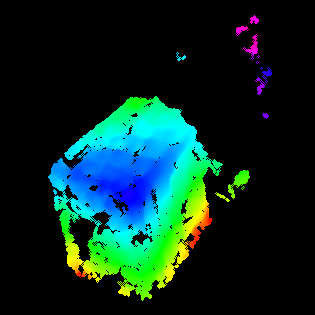
\includegraphics[width=95pt]{figures/visu_depth.png}
	\caption{Mélységinformáció}
  \end{subfigure}
\begin{subfigure}[b]{.32\linewidth}
	\centering
	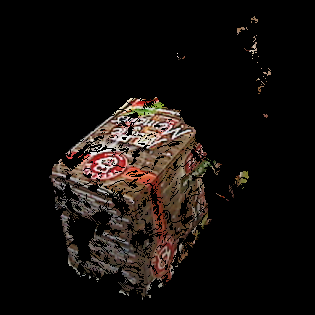
\includegraphics[width=95pt]{figures/visu_pixels.png}
	\caption{Eredeti pixelek}
  \end{subfigure}
\begin{subfigure}[b]{.32\linewidth}
	\centering
	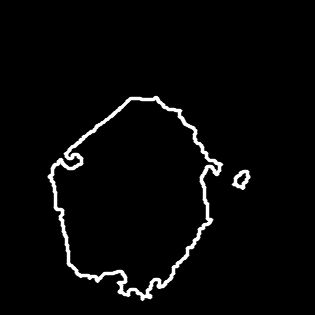
\includegraphics[width=95pt]{figures/visu_contours.png}
	\caption{Kontúrok}
  \end{subfigure}
\end{figure}

\end{frame}

\begin{frame}[c]{Nézőpont változtatása}

\only<1>{
\centering
\hspace{0pt}
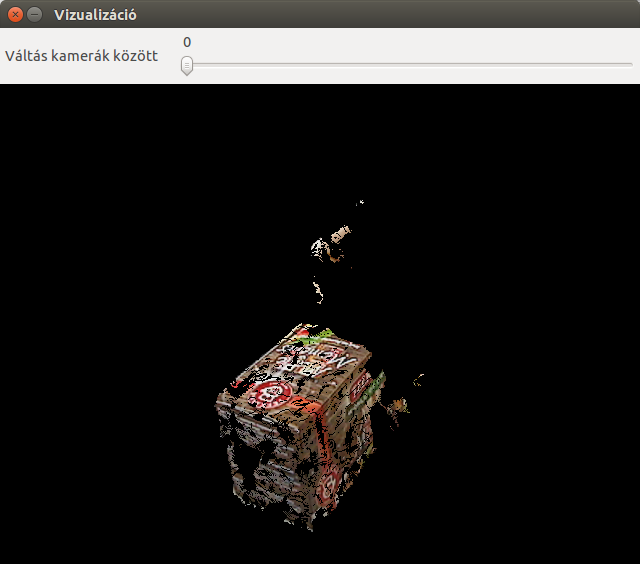
\includegraphics[width=230pt]{figures/visu_pixels_left.png}
}
\only<2>{
\centering
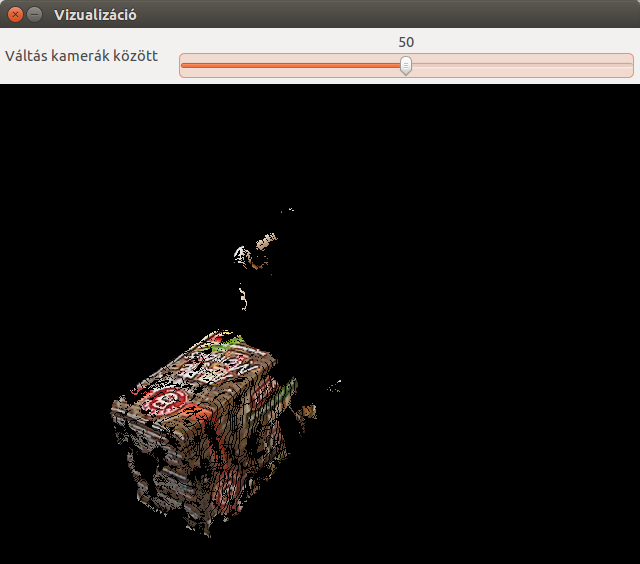
\includegraphics[width=230pt]{figures/visu_pixels_center.png}
}
\only<3>{
\centering
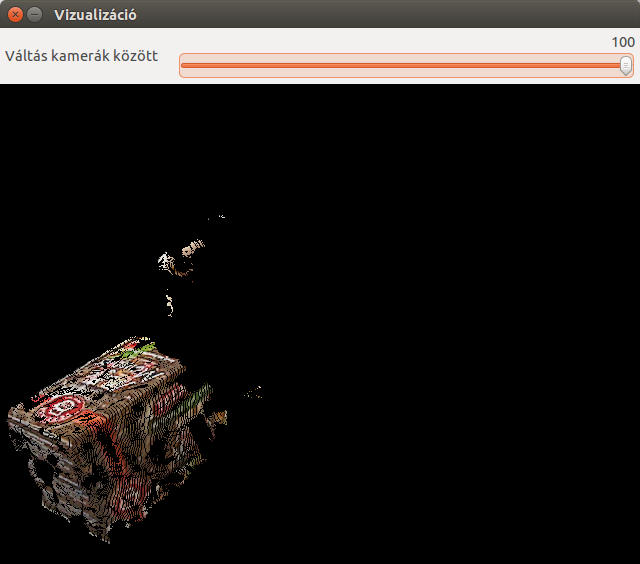
\includegraphics[width=230pt]{figures/visu_pixels_right.png}
}

\end{frame}

%----------------------------------------------------------------------------
\section[Eredmények]{Eredmények}
%----------------------------------------------------------------------------

\subsection{Három jelenet}
%----------------------------------------------------------------------------

\begin{frame}{1. jelenet}

\centering

\begin{figure}

\begin{subfigure}[b]{.32\linewidth}
	\centering
	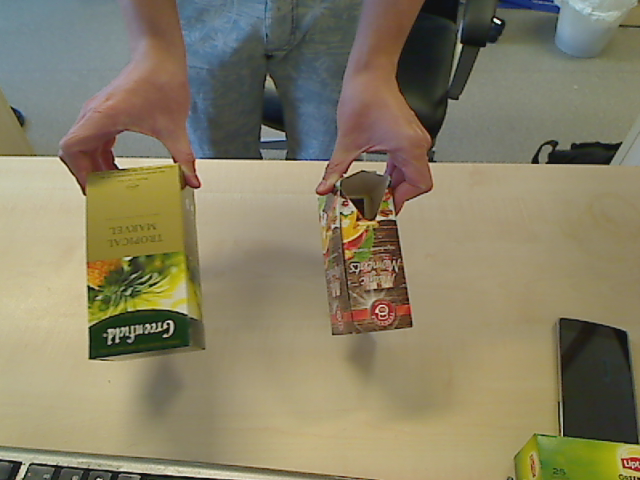
\includegraphics[width=95pt]{figures/left_93.png}
  \end{subfigure}
\begin{subfigure}[b]{.32\linewidth}
	\centering
	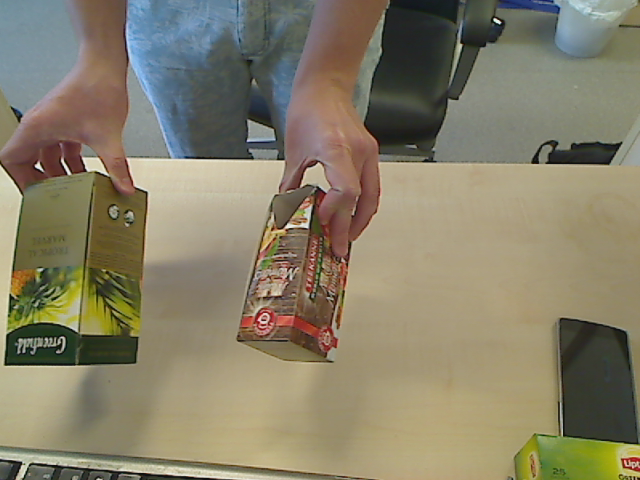
\includegraphics[width=95pt]{figures/left_153.png}
  \end{subfigure}
\begin{subfigure}[b]{.32\linewidth}
	\centering
	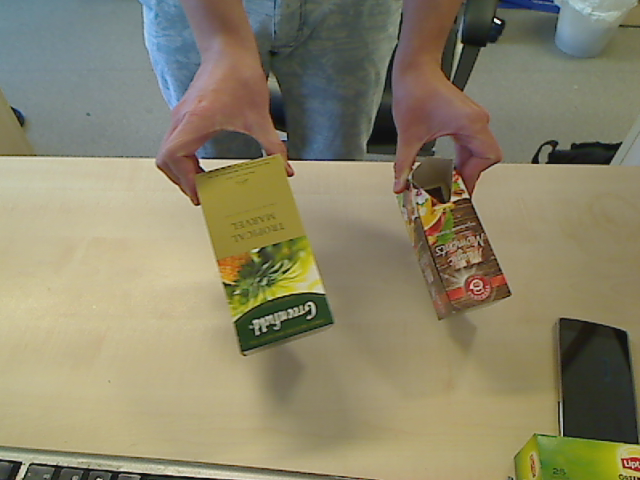
\includegraphics[width=95pt]{figures/left_223.png}
  \end{subfigure}\\\vspace{5pt}
\begin{subfigure}[b]{.32\linewidth}
	\centering
	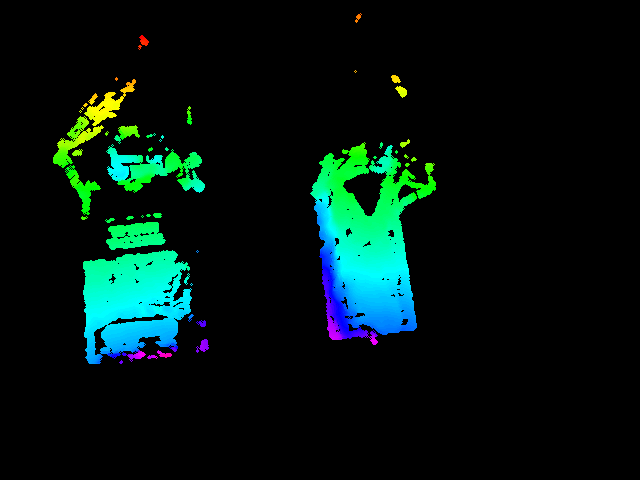
\includegraphics[width=95pt]{figures/vis_93.png}
  \end{subfigure}
\begin{subfigure}[b]{.32\linewidth}
	\centering
	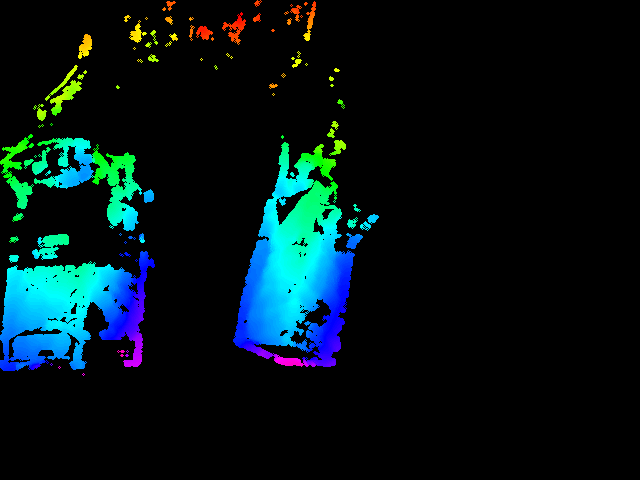
\includegraphics[width=95pt]{figures/vis_153.png}
  \end{subfigure}
\begin{subfigure}[b]{.32\linewidth}
	\centering
	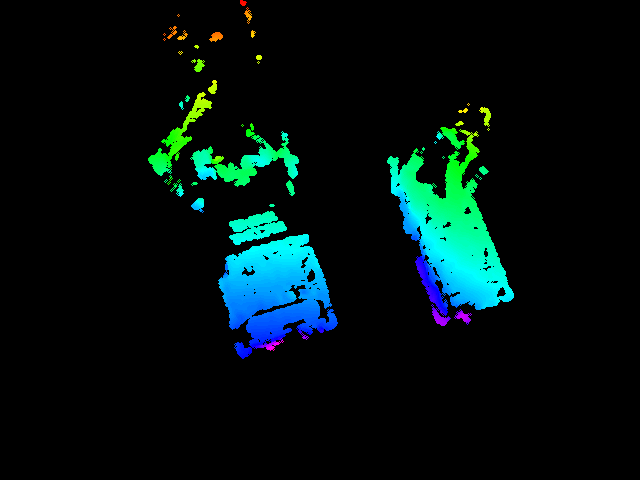
\includegraphics[width=95pt]{figures/vis_223.png}
  \end{subfigure}
  
\end{figure}

\end{frame}

\begin{frame}{2. jelenet}

\begin{figure}

\begin{subfigure}[b]{.32\linewidth}
	\centering
	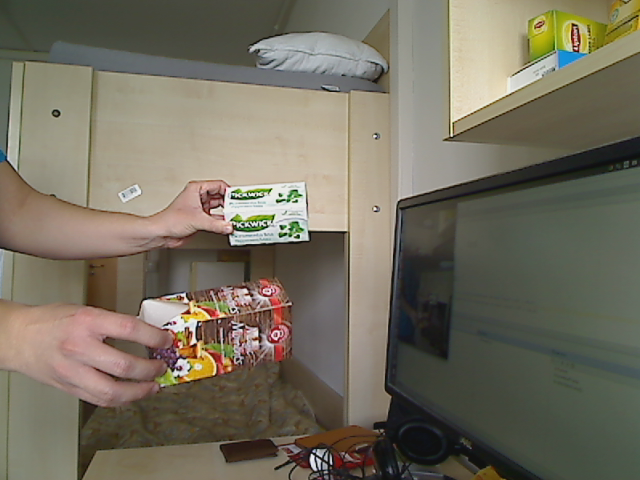
\includegraphics[width=95pt]{figures/scene2/left_45.png}
  \end{subfigure}
\begin{subfigure}[b]{.32\linewidth}
	\centering
	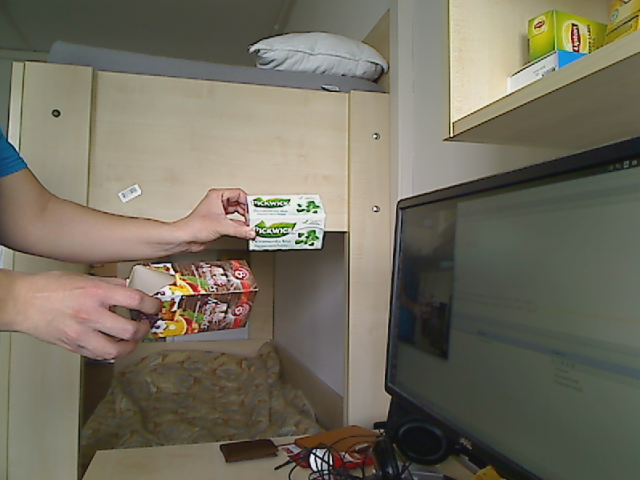
\includegraphics[width=95pt]{figures/scene2/left_130.png}
  \end{subfigure}
\begin{subfigure}[b]{.32\linewidth}
	\centering
	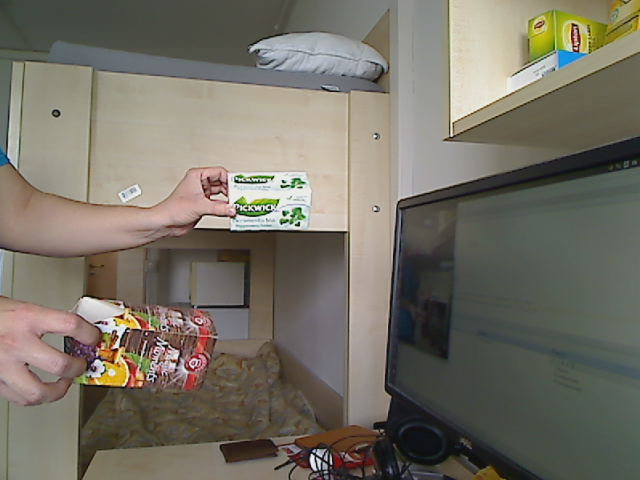
\includegraphics[width=95pt]{figures/scene2/left_215.png}
  \end{subfigure}\\\vspace{5pt}
\begin{subfigure}[b]{.32\linewidth}
	\centering
	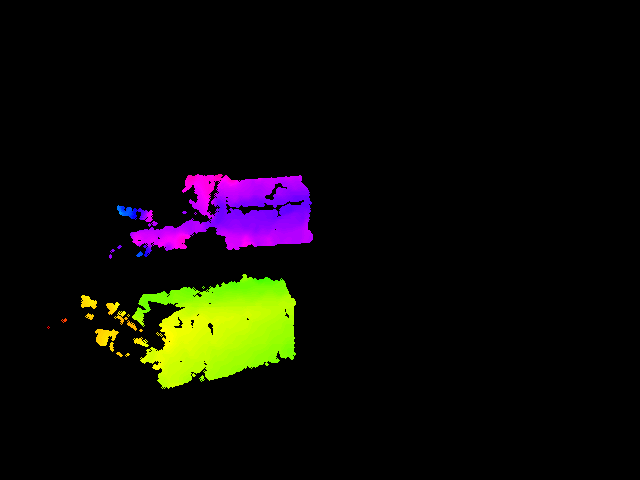
\includegraphics[width=95pt]{figures/scene2/vis_45.png}
  \end{subfigure}
\begin{subfigure}[b]{.32\linewidth}
	\centering
	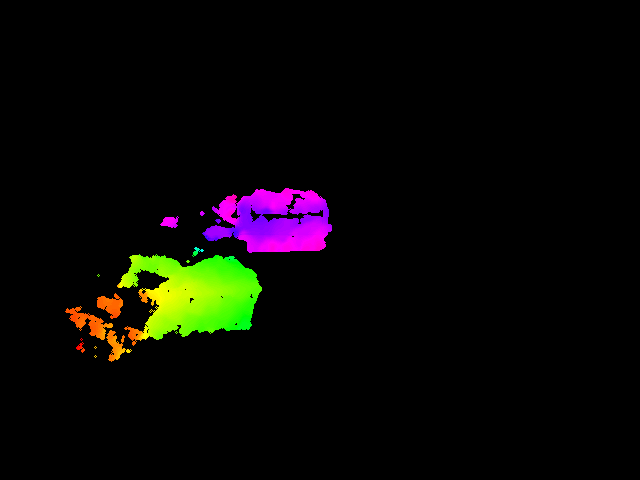
\includegraphics[width=95pt]{figures/scene2/vis_130.png}
  \end{subfigure}
\begin{subfigure}[b]{.32\linewidth}
	\centering
	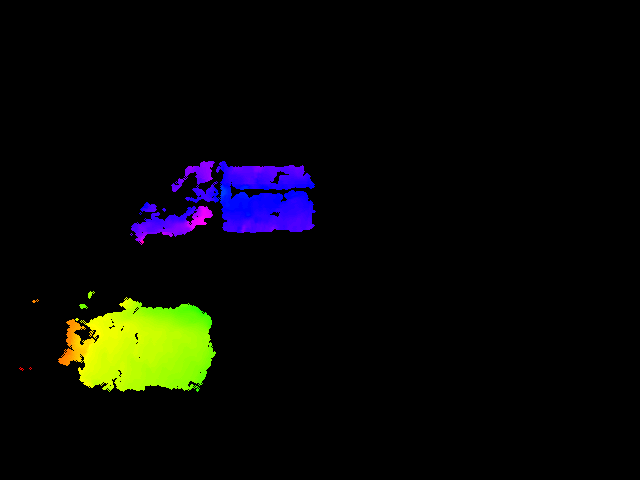
\includegraphics[width=95pt]{figures/scene2/vis_215.png}
  \end{subfigure}
  
\end{figure}


\end{frame}

\begin{frame}{3. jelenet}

\vspace{-13pt}
\begin{figure}
\centering
\begin{subfigure}[b]{.32\linewidth}
	\centering
	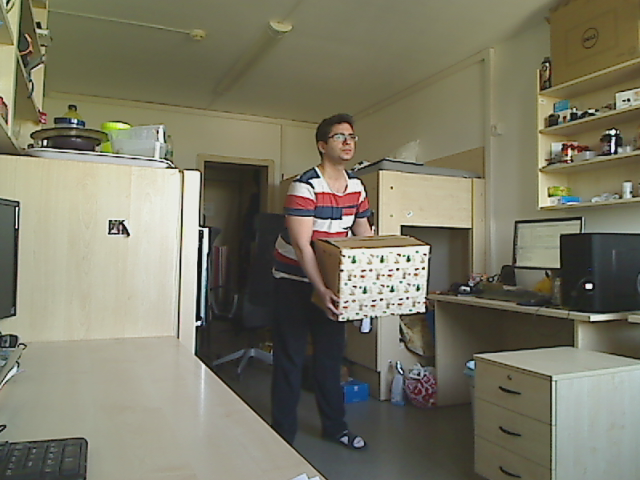
\includegraphics[width=90pt]{figures/scene3/left_152.png}
  \end{subfigure}
\begin{subfigure}[b]{.32\linewidth}
	\centering
	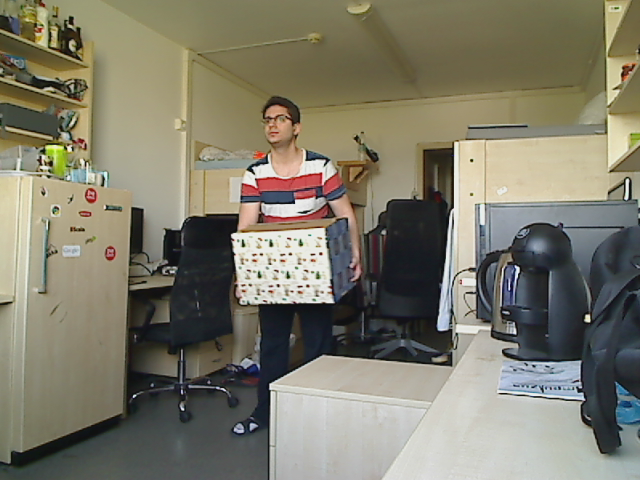
\includegraphics[width=90pt]{figures/scene3/right_152.png}
  \end{subfigure}
\begin{subfigure}[b]{.32\linewidth}
	\centering
	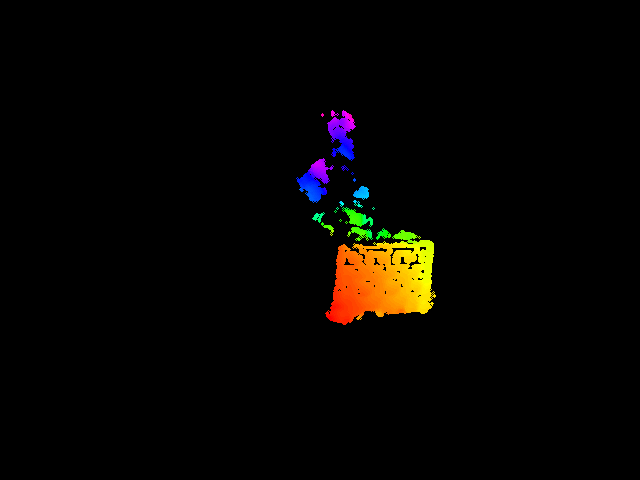
\includegraphics[width=90pt]{figures/scene3/vis_152.png}
  \end{subfigure}\\\vspace{3pt}
 \begin{subfigure}[b]{.32\linewidth}
	\centering
	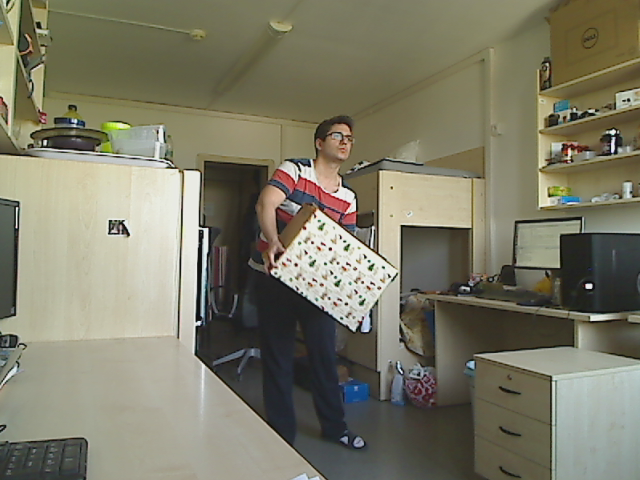
\includegraphics[width=90pt]{figures/scene3/left_196.png}
  \end{subfigure}
\begin{subfigure}[b]{.32\linewidth}
	\centering
	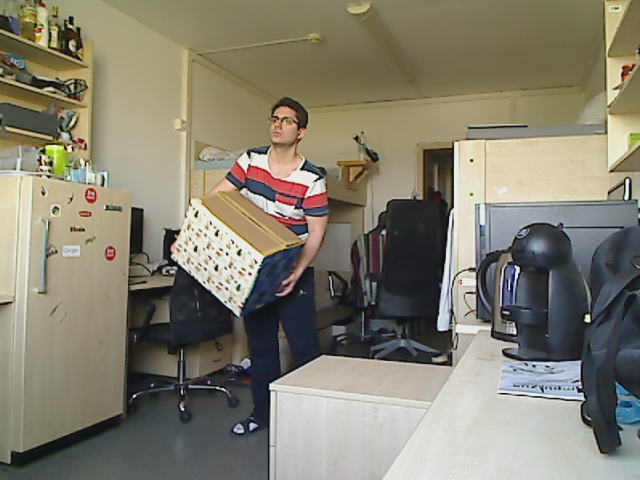
\includegraphics[width=90pt]{figures/scene3/right_196.png}
  \end{subfigure}
\begin{subfigure}[b]{.32\linewidth}
	\centering
	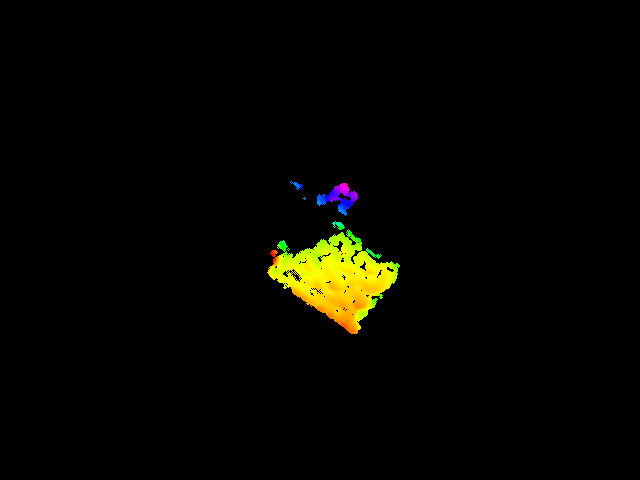
\includegraphics[width=90pt]{figures/scene3/vis_196.png}
  \end{subfigure}\\\vspace{3pt}
 \begin{subfigure}[b]{.32\linewidth}
	\centering
	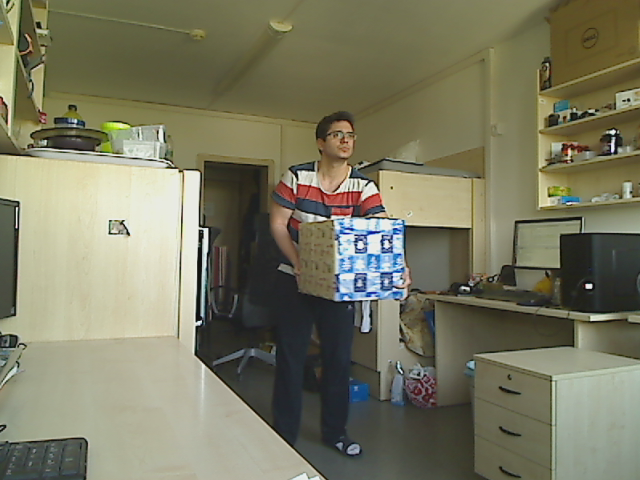
\includegraphics[width=90pt]{figures/scene3/left_376.png}
  \end{subfigure}
\begin{subfigure}[b]{.32\linewidth}
	\centering
	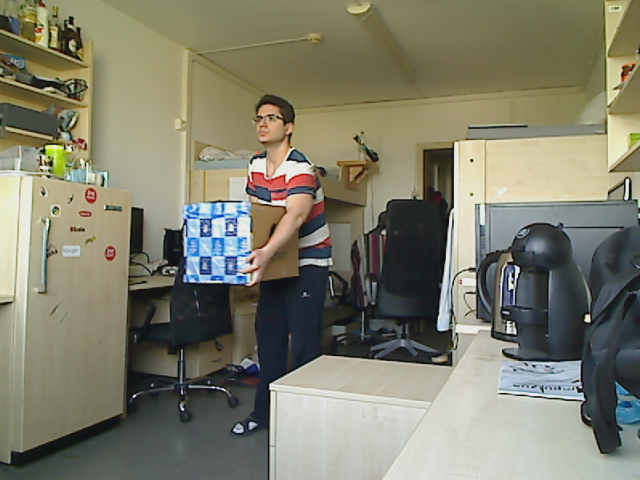
\includegraphics[width=90pt]{figures/scene3/right_376.png}
  \end{subfigure}
\begin{subfigure}[b]{.32\linewidth}
	\centering
	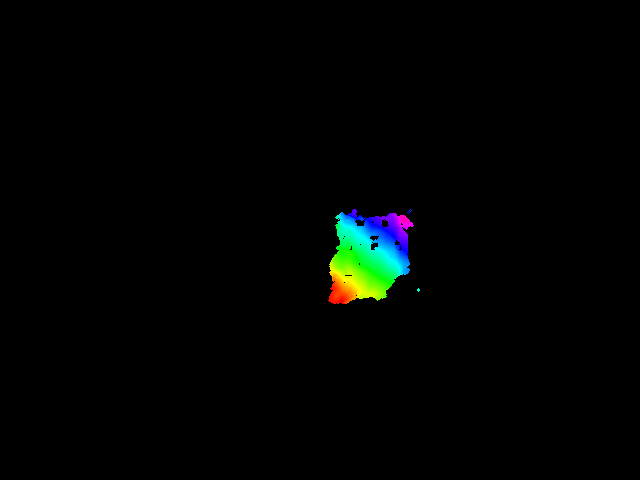
\includegraphics[width=90pt]{figures/scene3/vis_376.png}
  \end{subfigure}
\end{figure}

\end{frame}


\subsection{Valós idejű korlátok vizsgálata}
%----------------------------------------------------------------------------

\begin{frame}[c]{Kezdeti eredmények}

\centering
\begin{tabular}{|l|l|l|}
\hline
\textbf{Jelenet} & \textbf{Átlagos sebesség} & \textbf{Átlagos visszavetítési hiba} \\ \hline\hline

1. jelenet & 1,1 FPS & 0,8 pixel \\\hline
2. jelenet & 1,95 FPS & 1,5 pixel \\\hline
3. jelenet & 2,49 FPS & 2,54 pixel \\\hline
\end{tabular}

\end{frame}

\begin{frame}{Párhuzamosítás, GPU-n történő futtatás}

\begin{itemize}
\item párhuzamosítás: OpenMP
\begin{itemize}
\item maszkok meghatározása
\item oda-vissza optikai folyam
\item objektumok párhuzamos rekonstrukciója
\end{itemize}
\item GPU (OpenCV)
\begin{itemize}
\item optikai folyam
\item {\color{lightgray}jellegzetes pontok számolása (ORB)}
\end{itemize}
\end{itemize}

\end{frame}

\begin{frame}[c]{Végső eredmények}

\centering
\begin{tabular}{|l|l|l|}
\hline
\textbf{Módszer} & \textbf{Felbontás} & \textbf{Átlagos sebesség} \\ \hline\hline

1. jelenet  & $640\times 480$ & \textbf{3,86 FPS} \\ \hline\hline
2. jelenet & $640\times 480$ & \textbf{4,48 FPS} \\ \hline\hline
3. jelenet & $640\times 480$ & \textbf{6,06 FPS} \\ \hline\hline

1. jelenet, eredeti kép kicsinyítve & $320\times 240$ & 10,1 FPS \\ \hline
1. jelenet, eredeti kép kicsinyítve & $160\times 120$ & \textbf{14,3 FPS} \\ \hline\hline

1. jelenet, eredeti kép egy részlete & $320\times 240$ & 7,7 FPS \\ \hline
1. jelenet, eredeti kép egy részlete & $160\times 140$ & \textbf{12 FPS} \\ \hline

\end{tabular}

\end{frame}

%----------------------------------------------------------------------------
\section[Továbbfejlesztés]{Továbbfejlesztési lehetőségek}
%----------------------------------------------------------------------------
  
  
  \begin{frame}{Továbbfejlesztési lehetőségek}
    \begin{itemize}
      \item más, gyorsabb optikai folyam algoritmus kipróbálása
      \item maszkok meghatározása jó, de \textit{lassú}: más módszer?
      \item egyéb műveletek is GPU-n
      \begin{itemize}
      \item pl. textúrázottság ellenőrzése
      \item OpenCL az OpenCV-ben
      \end{itemize}
      \item felületek meghatározása és textúrázása
    \end{itemize}
  \end{frame}


%----------------------------------------------------------------------------
\section{Összefoglalás}
%----------------------------------------------------------------------------
  \begin{frame}{Összefoglalás}
    \begin{itemize}
      \justifying
      \item elméleti háttér
      \item szimulációs szoftver
      \begin{itemize}
      \item tervezés
      \item implementálás (+gyorsítás)
      \item tesztelés három jeleneten
      \end{itemize}
      \item valós idejű korlátok vizsgálata
      \begin{itemize}
        \item nem 24 képkocka másodpercenként
        \item de már gyakorlatban használható
      \end{itemize}
    \end{itemize}
  \end{frame}
  